\documentclass[diploma]{SCWorks}
% Тип обучения (одно из значений):
%    bachelor   - бакалавриат (по умолчанию)
%    spec       - специальность
%    master     - магистратура
% Форма обучения (одно из значений):
%    och        - очное (по умолчанию)
%    zaoch      - заочное
% Тип работы (одно из значений):
%    coursework - курсовая работа (по умолчанию)
%    referat    - реферат
%  * otchet     - универсальный отчет
%  * nirjournal - журнал НИР
%  * digital    - итоговая работа для цифровой кафдры
%    diploma    - дипломная работа
%    pract      - отчет о научно-исследовательской работе
%    autoref    - автореферат выпускной работы
%    assignment - задание на выпускную квалификационную работу
%    review     - отзыв руководителя
%    critique   - рецензия на выпускную работу
% Включение шрифта
%    times      - включение шрифта Times New Roman (если установлен)
%                 по умолчанию выключен
\usepackage{preamble}
% \captionsetup[figure]{font= normalsize, labelfont=normalsize}
\renewcommand\theFancyVerbLine{\small\arabic{FancyVerbLine}}

\begin{document}

% Кафедра (в родительном падеже)
\chair{математической кибернетики и компьютерных наук}

% Тема работ
\title{Разработка web-приложения для организации
процесса уборки мусора}

% Курс
\course{4}

% Группа
\group{451}

% Факультет (в родительном падеже) (по умолчанию "факультета КНиИТ")
% \department{факультета КНиИТ}

% Специальность/направление код - наименование
% \napravlenie{02.03.02 "--- Фундаментальная информатика и информационные технологии}
% \napravlenie{02.03.01 "--- Математическое обеспечение и администрирование информационных систем}
% \napravlenie{09.03.01 "--- Информатика и вычислительная техника}
\napravlenie{09.03.04 "--- Программная инженерия}
% \napravlenie{10.05.01 "--- Компьютерная безопасность}

% Для студентки. Для работы студента следующая команда не нужна.
% \studenttitle{Студентки}

% Фамилия, имя, отчество в родительном падеже
\author{Устюшина Богдана Антоновича}

% Заведующий кафедрой 
\chtitle{доцент, к.\,ф.-м.\,н.}
\chname{С.\,В.\,Миронов}

% Руководитель ДПП ПП для цифровой кафедры (перекрывает заведующего кафедры)
% \chpretitle{
%     заведующий кафедрой математических основ информатики и олимпиадного\\
%     программирования на базе МАОУ <<Ф"=Т лицей №1>>
% }
% \chtitle{г. Саратов, к.\,ф.-м.\,н., доцент}
% \chname{Кондратова\, Ю.\,Н.}

% Научный руководитель (для реферата преподаватель проверяющий работу)
\satitle{доцент, к.\,ф.-м.\,н.} %должность, степень, звание
\saname{А.\,С.\,Иванов}

% Руководитель практики от организации (руководитель для цифровой кафедры)
\patitle{доцент, к.\,ф.-м.\,н.}
\paname{С.\,В.\,Миронов}

% Руководитель НИР
\nirtitle{доцент, к.\,п.\,н.} % степень, звание
\nirname{В.\,А.\,Векслер}

% Семестр (только для практики, для остальных типов работ не используется)
\term{2}

% Наименование практики (только для практики, для остальных типов работ не
% используется)
\practtype{учебная}

% Продолжительность практики (количество недель) (только для практики, для
% остальных типов работ не используется)
\duration{2}

% Даты начала и окончания практики (только для практики, для остальных типов
% работ не используется)
\practStart{01.07.2022}
\practFinish{13.01.2023}

% Год выполнения отчета
\date{2025}

\maketitle

% Включение нумерации рисунков, формул и таблиц по разделам (по умолчанию -
% нумерация сквозная) (допускается оба вида нумерации)
% \secNumbering

\tableofcontents

% Раздел "Обозначения и сокращения". Может отсутствовать в работе
% \abbreviations
% \begin{description}
%     \item ... "--- ...
%     \item ... "--- ...
% \end{description}

% Раздел "Определения". Может отсутствовать в работе
% \definitions

% Раздел "Определения, обозначения и сокращения". Может отсутствовать в работе.
% Если присутствует, то заменяет собой разделы "Обозначения и сокращения" и
% "Определения"
% \defabbr

\sloppy

\intro

В современном мире проблема загрязнения окружающей среды становится всё более 
актуальной, и мусор, оставляемый на улицах, представляет собой одну из самых 
серьёзных составляющих этой проблемы. Накопление отходов в общественных местах 
не только нарушает эстетический облик городов, но и оказывает негативное 
воздействие на здоровье человека и окружающую экосистему. С каждым годом 
количество бытового и промышленного мусора растёт, и его присутствие на 
улицах городов становится всё более заметным. Это вызывает множество проблем, 
от ухудшения качества воздуха до разрушения экосистем и негативного влияния 
на биоразнообразие.

Мусор, оставляемый на улицах, становится источником различных заболеваний, так 
как разлагающиеся отходы выделяют вредные вещества в воздух и почву. 
Загрязнение воздуха, вызванное гниением мусора, может приводить к серьёзным 
проблемам со здоровьем, таким как аллергические реакции и респираторные 
заболевания. Кроме того, скопление мусора привлекает животных и насекомых, 
что может стать причиной распространения инфекционных заболеваний. Каждый 
элемент уличного мусора, будь то пластиковая бутылка, упаковка или другие 
отходы, способен оказать разрушительное влияние на окружающую среду, нарушая 
естественные экосистемные процессы и угрожая существованию многих видов 
растений и животных.

Ситуация с утилизацией мусора на улицах становится всё более серьёзной. 
Местные власти часто не успевают оперативно реагировать на проблемы, связанные 
с накоплением отходов, из-за нехватки ресурсов и информации о местах их 
скопления. В то же время, население не всегда осведомлено о правильных 
способах утилизации мусора и необходимости поддержания чистоты в своём 
окружении. Поэтому крайне важно не только повышать уровень экологической 
осведомлённости граждан, но и предоставлять им удобные инструменты для 
сообщения о проблемах, связанных с мусором на улицах.

Современные технологии, особенно мобильные приложения, могут стать важным 
инструментом в борьбе с проблемой мусора на улицах. Мобильные платформы 
позволяют быстро и эффективно информировать местные власти о проблемах с 
загрязнением, а также организовывать взаимодействие между гражданами и 
ответственными службами. В рамках своей курсовой работы я разрабатываю 
приложение, которое позволит жителям оперативно сообщать о местах, где 
скопился мусор на улицах, и помогать ответственным службам быстрее устранять 
эти нарушения.

Моё приложение станет платформой для гражданского взаимодействия, где каждый 
пользователь сможет внести свой вклад в улучшение чистоты в своём городе. 
Пользователи смогут легко отправлять сообщения о местах накопления мусора, 
включая фотографии и описание проблемы. Это даст возможность ответственным 
службам более оперативно реагировать на обращения граждан и принимать меры по 
устранению мусора.

Такой подход позволит создать активное сообщество, заинтересованное в 
поддержании чистоты на улицах. Приложение будет не только инструментом для 
сообщения о проблемах, но и средством повышения осведомлённости населения о 
важности заботы о чистоте окружающей среды. Я надеюсь, что благодаря таким 
инициативам мы сможем привлечь внимание к проблеме мусора на улицах и внести 
реальный вклад в её решение, создавая чистую и здоровую среду для будущих 
поколений.

Целью работы является разработка web-приложения для эффективной организации
процесса нахождения и уборки мусора на улицах города. Также планируется сделать
упор на создание чистой архитектуры приложения и построение 
масштабируемой системы. Конечно, сегодня для построения такой масштабируемой и 
отказоустойчивой системы используется подход с микросервисной архитектурой, 
однако в рамках дипломной работы для ограничения сложности проекта, а также
из-за небольшого масштаба самого проекта было принято решение в сторону
монолитной архитектуры при разработке backend-сервиса.

Таким образом, для достижения цели необходимо решить следующие задачи:
\begin{enumerate}
    \item рассмотреть используемые технологии, описать преимущества выбранного 
    стека;
    \item описать архитектуру и структуру построенной информационной системы, 
    database-, backend- и frontend-сервисов, а также описать основные решения
    дизайна архитектуры;
    \item реализовать это с помощью выбранных инструментов.
\end{enumerate}

\section{Обзор используемых инструментов}

При разработке современных веб-приложений крайне важно выбирать
надёжные и производительные технологии, которые обеспечат 
масштабируемость, гибкость и лёгкость в обслуживании проекта. 
В своём проекте я использую следующие технологии:
\begin{enumerate}
    \item PostgreSQL в качестве реляционной базы данных;
    \item Golang c web-фреймворком Gin для разработки серверного приложения;
    \item React в качестве frontend-фреймворка для разработки клиентского 
    приложения;
    \item Docker и docker compose как современный (де-факто) стандарт 
    контейнеризации и автоматизации деплоя приложения.
    \item концепция JSON Web Token (JWT) вместе с идеей парных токенов (access-
    и refresh) для построение системы авторизации пользователей.
\end{enumerate}

Также вот список основных библиотек, используемых в моей дипломной работе:
\begin{enumerate}
    \item Backend
    \begin{itemize}
        \item Gin-gonic
        \item Gin-swagger
        \item Squirrel
    \end{itemize}
    \item Frontend
    \begin{itemize}
        \item React
        \item React Router 
        \item Radix UI
        \item Shadcn/ui
    \end{itemize}
\end{enumerate}

Следует отметить, что важны не только инструменты, которые непосредственно 
создают информационную систему, но и те, которые помогают в процессе разработки.
В рамках работы я использовал следующие инструменты:
\begin{enumerate}
    \item DBeaver в качестве интерфейса для работы с базой данных;
    \item Postman для автоматизации тестирования API, который впоследствии будет
    использовать клиент;
    \item Air для hot-reload сервера;
    \item Goose для автоматизации накатки миграций;
    \item Swag для автогенерации документации API;
    \item Vite и Yarn для сборки и управления зависимостями.
\end{enumerate}

У всего вышеописанного есть важные преимущества, которые делают 
их достойными для создания стабильной, эффективной и масштабируемой системы. 
Рассмотрим более подробно, почему стоит выбрать эти инструменты для разработки.

\subsection{Инструменты построения информационной системы}

\subsubsection{Golang}

Язык программирования Go (часто также называемый Golang) был разработан 
с целью устранения некоторых проблем, наблюдаемых в 
существующих на тот момент языках программирования, таких как C, C++, Java 
и других. Основной задачей, которую ставили перед собой разработчики Go, 
было создание языка, сочетающего в себе простоту синтаксиса, высокую 
производительность и встроенную поддержку параллельных вычислений, что 
особенно важно в эпоху масштабируемых распределённых систем и облачных 
вычислений.

В конечном итоге Go стал языком следующего поколения после Java, C\# и C++, 
которые в начале нулевых были одними из главных для продуктовой разработки. 
Go представляет собой компилируемый, строго типизированный язык 
программирования, ориентированный на разработку высоконагруженных серверных 
приложений. Одной из ключевых концепций языка является простота: синтаксис 
Go достаточно лаконичен, но при этом выразителен, что делает его доступным 
как для начинающих, так и для опытных программистов. В отличие от более 
сложных языков, в которых существует множество парадигм и способов достижения 
одной и той же цели, Go стремится к единообразию и предсказуемости кода, 
что значительно облегчает его сопровождение и коллективную разработку.

Среди основных преимуществ языка Go можно выделить следующие:
\begin{enumerate}
    \item Благодаря тому, что Go является компилируемым языком, программы на 
    Go выполняются с производительностью, сопоставимой с C/C++. Это делает 
    его особенно привлекательным для разработки системного программного 
    обеспечения и высоконагруженных сервисов.
    \item Язык Go содержит минимально необходимый набор конструкций, 
    избавленный от избыточности. В Go отсутствует наследование, перегрузка 
    операторов, обобщения (до версии 1.18), а также множество других сложных 
    особенностей, характерных для многих современных языков. Это способствует 
    упрощению кода и снижению вероятности ошибок.
    \item Одной из самых мощных возможностей Go является встроенная модель 
    конкурентности, реализованная через горутины и каналы. Горутины 
    представляют собой легковесные потоки, которые создаются и управляются 
    на уровне runtime языка, что делает возможным выполнение множества 
    параллельных задач без значительных затрат ресурсов.
    \item Go предоставляет обширную стандартную библиотеку, включающую 
    инструменты для работы с сетью, HTTP, строками, файлами, форматированием 
    и другими важнейшими аспектами программной разработки. Это позволяет 
    создавать полнофункциональные приложения без необходимости подключения 
    сторонних зависимостей.
    \item Приложения на Go компилируются в статически связанные исполняемые 
    файлы, что упрощает их развёртывание и интеграцию в различные среды. 
    Такая особенность особенно актуальна при разработке микросервисов и 
    контейнеризованных решений.
    \item Go позволяет легко собирать исполняемые файлы под разные 
    операционные системы и архитектуры, просто указав соответствующую 
    переменную окружения. Это делает Go удобным для разработки 
    кроссплатформенных приложений и сервисов.
\end{enumerate}

Что касается областей применения языка Go, то они весьма разнообразны. На 
сегодняшний день Go широко используется в разработке:
\begin{enumerate}
    \item высоконагруженных веб-серверов и REST API;
    \item микросервисных архитектур и облачных решений;
    \item инструментов для DevOps и автоматизации (в том числе широко 
    известных — Docker, Kubernetes, Terraform написаны на Go);
    \item сетевого программного обеспечения и прокси-серверов;
    \item распределённых систем, требующих масштабируемости и высокой надёжности;
    \item системного ПО, в том числе CLI-приложений и утилит.
\end{enumerate}
    
Одним из решающих факторов при выборе Go в рамках настоящего дипломного 
проекта стало сочетание производительности, простоты и удобства при 
построении серверной части веб-приложения. Go предоставляет разработчику все 
необходимые средства для быстрой реализации HTTP-серверов, маршрутизации, 
сериализации и обработки запросов, что делает его особенно привлекательным 
для backend-разработки. Кроме того, строгая типизация языка способствует 
повышению надёжности программного кода и снижению числа потенциальных ошибок 
на этапе выполнения \cite{go-docs,go-by-example}.

\subsubsection{React}

React (или React.js) представляет собой современную JavaScript-библиотеку с 
открытым исходным кодом. Основное предназначение React — упрощение процесса 
создания пользовательских интерфейсов, особенно в контексте одностраничных 
приложений (SPA), где требуется динамически изменять содержимое страницы без 
её полной перезагрузки.

React был представлен в 2013 году и с тех пор приобрёл широкую популярность 
в профессиональной среде, благодаря своей компонентной архитектуре, высокой 
производительности и активной поддержке со стороны сообщества разработчиков.

В основе React лежит идея декларативного программирования, при котором 
разработчик описывает то, что должно быть отображено, а не как именно это 
должно быть сделано. Такой подход упрощает понимание логики интерфейса и 
делает код более читаемым и сопровождаемым.

Ключевыми преимуществами React являются:

\begin{itemize}
    \item React поощряет разбиение интерфейса на переиспользуемые, независимые 
    компоненты, что упрощает разработку, тестирование и сопровождение крупных 
    приложений. Каждый компонент инкапсулирует собственную логику и визуальное 
    представление.
    \item React использует внутреннее представление DOM-дерева в памяти 
    (виртуальный DOM), которое позволяет минимизировать количество операций 
    обновления реального DOM, что значительно ускоряет работу интерфейса, 
    особенно при большом объёме данных.
    \item Передача данных от родительских компонентов к дочерним 
    осуществляется в одном направлении, что делает поведение интерфейса 
    более предсказуемым и снижает вероятность ошибок, связанных с 
    неконтролируемыми изменениями состояния.
    \item React активно использует новейшие возможности языка JavaScript, 
    такие как стрелочные функции, деструктуризация, модули, классы и т.\,д., 
    что способствует написанию более лаконичного и выразительного кода.
    \item React легко интегрируется с другими библиотеками и инструментами 
    (Redux, React Router, Axios, и т.\,д.), что позволяет гибко строить 
    архитектуру приложения в соответствии с конкретными требованиями проекта.
    \item Благодаря таким инструментам, как Next.js, React может 
    использоваться не только для клиентской, но и для серверной генерации 
    страниц, что повышает SEO-дружественность и производительность 
    веб-приложений.
\end{itemize}

На сегодняшний день React широко используется для создания:

\begin{itemize}
    \item одностраничных веб-приложений (SPA);
    \item административных панелей и систем управления контентом;
    \item интернет-магазинов и интерфейсов электронной коммерции;
    \item мобильных приложений (через React Native);
    \item внутренних корпоративных платформ;
    \item систем мониторинга и визуализации данных.
\end{itemize}

В контексте настоящего дипломного проекта использование React обусловлено 
необходимостью создания гибкого, отзывчивого и масштабируемого 
пользовательского интерфейса, который способен динамически взаимодействовать 
с backend-сервисом. Компонентный подход и использование виртуального DOM 
позволяют эффективно управлять состоянием приложения и обеспечивать высокую 
скорость отклика. Кроме того, активная поддержка сообщества и богатая 
документация делают React надёжным выбором при разработке современных 
веб-приложений \cite{react-docs,react-mdn}.

\subsubsection{PostgreSQL}

PostgreSQL — это мощная объектно-реляционная система управления 
базами данных (СУБД), которая на протяжении многих лет остаётся 
одним из лидеров среди open-source решений для работы с данными. 
В своём проекте я использую PostgreSQL, и на это есть несколько причин:

PostgreSQL славится своей надёжностью и стабильностью.
Она предоставляет высокую степень защиты данных и обеспечивает 
устойчивость к сбоям, что делает её идеальной для критически 
важных приложений, требующих максимальной сохранности информации.

PostgreSQL отлично масштабируется и поддерживает работу с большими
объёмами данных. Это важное преимущество для приложений, 
которые планируются к расширению в будущем, или для тех, кто 
работает с массивами данных в реальном времени.

В отличие от некоторых других реляционных СУБД, PostgreSQL
поддерживает не только стандартные реляционные структуры данных, 
но и работу с JSON, геоданными, используя технологию PostGIS 
и другими сложными типами данных. Это делает её особенно полезной 
для приложений, которые требуют гибкости в работе с 
разнообразными структурами данных.

PostgreSQL полностью соответствует стандартам SQL, что делает 
её совместимой с большим количеством других систем и инструментов. 
Это позволяет использовать её в самых разных проектах и легко 
переносить на неё существующие базы данных.

PostgreSQL обеспечивает полную поддержку транзакций, что гарантирует 
целостность данных и их сохранность в случае сбоев. Это особенно 
важно для приложений, работающих с финансовыми данными или 
другими критически важными ресурсами.

PostgreSQL является бесплатной и открытой СУБД с огромным
сообществом разработчиков и пользователей. Это не только 
экономически выгодно, но и позволяет гибко настраивать систему 
под конкретные нужды проекта \cite{postgresql}.

\subsubsection{Docker}

Docker — это платформа для автоматизации развёртывания приложений 
в контейнерах. Контейнеризация позволяет упаковать приложение и 
все его зависимости в единый контейнер, что гарантирует его работу 
в любой среде. Docker стал неотъемлемой частью современных процессов 
разработки и развертывания благодаря своим многочисленным преимуществам.

Одним из ключевых преимуществ Docker является возможность создания 
изолированных контейнеров, в которых выполняется приложение. 
Это означает, что разработчик может быть уверен, что приложение 
будет работать одинаково на любой машине, независимо от её операционной 
системы и установленных зависимостей. Изоляция помогает избежать 
проблем, связанных с несовместимостью версий библиотек или конфигураций 
операционной системы.
    
Docker-контейнеры представляют собой лёгкие и переносимые единицы, 
которые можно запускать на любом сервере или облачном провайдере, 
поддерживающем Docker. Это делает приложение независимым от 
инфраструктуры, на которой оно работает, и упрощает перенос с локального 
окружения на серверное. При необходимости легко масштабировать 
приложение, запуская несколько контейнеров на разных узлах.
    
Docker идеально подходит для масштабирования микросервисов и 
распределённых систем. Контейнеры можно легко запускать параллельно, 
что позволяет масштабировать отдельные компоненты приложения в 
зависимости от нагрузки. Это также упрощает поддержку высокой 
доступности и балансировки нагрузки.
    
В отличие от виртуальных машин, которые требуют отдельного ядра 
операционной системы для каждого экземпляра, Docker использует 
ресурсы хоста, что делает контейнеры более лёгкими и менее 
ресурсоёмкими. Это позволяет запускать большее количество контейнеров 
на одном сервере по сравнению с виртуальными машинами.
    
Docker позволяет быстро разворачивать контейнеры, что значительно ускоряет 
процесс деплоя. Контейнеры можно легко обновлять, создавать новые версии 
образов и откатываться к предыдущим версиям при необходимости. Это даёт 
разработчикам и администраторам системы гибкость в управлении версиями 
приложения.
    
Docker позволяет описывать инфраструктуру через Dockerfile, где подробно 
указываются все этапы сборки образа, включая установку зависимостей, 
конфигурацию среды и подготовку приложения к запуску. Это даёт возможность 
легко автоматизировать процесс сборки и развертывания, делая его 
воспроизводимым.
    
Docker имеет огромное сообщество и развивающуюся экосистему. Существует 
множество готовых к использованию контейнеров в Docker Hub, что позволяет 
значительно ускорить процесс разработки за счёт использования существующих 
решений, таких как базы данных, кэш-системы, и другие сервисы.

\subsubsection{Docker Compose}

В дополнение к Docker я также использую Docker Compose. Docker Compose — это 
инструмент для управления многоконтейнерными приложениями, который изначально
являлся дополнением к контейнерной экосистеме Docker.

Docker Compose позволяет определять и запускать несколько контейнеров Docker 
как единое приложение, что упрощает настройку, управление и масштабирование 
сложных систем. Docker Compose использует файл конфигурации YAML для описания 
всех сервисов, их зависимостей, сетей и томов, необходимых для корректной 
работы приложения.

Docker Compose даёт возможность запускать одновременно несколько контейнеров, 
которые взаимодействуют друг с другом. Например, в рамках одного проекта могут 
быть контейнеры для веб-сервера, базы данных, кеширования и других сервисов. 
Это особенно полезно для микросервисной архитектуры, где каждое приложение 
состоит из множества взаимосвязанных компонентов.
    
Docker Compose использует понятный файл конфигурации 
\texttt{docker-compose.yml}, где описываются все сервисы, их зависимости и 
параметры запуска. Это позволяет легко управлять сложной инфраструктурой и 
делиться конфигурацией с другими разработчиками. Кроме того, этот файл делает 
инфраструктуру воспроизводимой: любой разработчик может развернуть такую же 
среду у себя локально, используя один и тот же конфигурационный файл.
    
Compose значительно упрощает разработку и тестирование многосоставных 
приложений. С его помощью можно настроить различные окружения (например, 
тестовые и продакшн) с минимальными усилиями. Разработчики могут быстро 
развернуть все необходимые компоненты в контейнерах, не настраивая вручную 
каждую службу.
    
Docker Compose упрощает работу с сетями, что важно для взаимодействия между 
контейнерами. Каждый сервис может находиться в отдельной сети или общаться с 
другими сервисами через виртуальные сети Docker. Это позволяет создавать 
изолированные окружения для разных частей приложения и управлять доступом 
между ними. Кроме того, Docker Compose позволяет настраивать постоянные тома 
для хранения данных, что критически важно для баз данных и других сервисов, 
требующих сохранения состояния.
    
Docker Compose позволяет легко масштабировать приложение, увеличивая 
количество реплик определённых контейнеров. Например, если веб-сервер начинает 
испытывать высокую нагрузку, его можно масштабировать до нескольких экземпляров 
без необходимости изменения конфигурации всего проекта. Это делает 
Docker Compose отличным инструментом для управления как разработкой, так и 
продакшн-средами.
    
Docker Compose может быть легко интегрирован в конвейеры непрерывной 
интеграции и доставки (CI/CD), что делает его полезным не только для 
локальной разработки, но и для автоматизированного развертывания приложений. 
С его помощью можно легко тестировать приложение в среде, максимально 
приближённой к продакшн.
    
Одно из важнейших преимуществ Docker Compose — это возможность запускать весь 
проект одной командой: \texttt{docker compose up}. Все необходимые контейнеры 
будут автоматически развернуты и запущены, что значительно ускоряет и упрощает 
процесс настройки окружения, особенно для новых разработчиков или тестировщиков.
    
Docker Compose предоставляет удобные инструменты для мониторинга состояния 
контейнеров, их логов и работы в целом. Это упрощает отладку приложений и 
позволяет своевременно находить и устранять возможные проблемы \cite{docker}.

\subsubsection{Авторизация}

JSON Web Token (JWT) — это компактный и безопасный формат представления 
информации между двумя сторонами в виде JSON-объекта, предназначенный 
преимущественно для передачи аутентификационных и авторизационных данных. 
JWT является частью спецификаций семейства JOSE (JSON Object Signing and 
Encryption) и широко используется в современных распределённых веб-приложениях 
для реализации механизма беззависимой (stateless) аутентификации.

В отличие от традиционных методов, таких как хранение пользовательской сессии 
на стороне сервера, JWT позволяет переносить всю необходимую информацию о 
пользователе непосредственно в токене, который хранится на клиенте. Это 
упрощает масштабирование системы, снижает нагрузку на backend и исключает 
необходимость централизованного хранилища сессий.

Каждый JWT состоит из трёх логически отделённых частей, разделённых точками:

\begin{enumerate}
    \item \textbf{Header} — заголовок, указывающий алгоритм подписи (например, 
    HS256) и тип токена.
    \item \textbf{Payload} — полезная нагрузка, содержащая утверждения 
    (\textit{claims}), такие как идентификатор пользователя, время истечения 
    срока действия токена, его роль и другие метаданные.
    \item \textbf{Signature} — цифровая подпись, формируемая на основе 
    закодированного заголовка и полезной нагрузки с использованием указанного 
    алгоритма и секретного ключа (или пары открытый/закрытый ключ при 
    использовании асимметричной криптографии).
\end{enumerate}

Пример структуры JWT в кодированном виде:

\begin{verbatim}
eyJhbGciOiJIUzI1NiIsInR5cCI6IkpXVCJ9.
eyJ1c2VyX2lkIjoxMjMsInJvbGUiOiJhZG1pbiJ9.
dBjftJeZ4CVP-mB92K27uhbUJU1p1r_wW1gFWFOEjXk
\end{verbatim}

Применение JWT обладает рядом очевидных преимуществ:

\begin{itemize}
    \item Серверу не требуется хранить сессионные данные, поскольку токен 
    содержит всю необходимую информацию. Это позволяет говорить о беззависимой
    (stateless) аутентификации.
    \item Возможность использования JWT делает систему более масштабируемой и 
    удобной в распределённых архитектурах (например, микросервисах)
    \item Токены представляют собой строки, удобные для передачи в 
    HTTP-заголовках или URL.
    \item Использование подписей (и при необходимости — шифрования) позволяет 
    гарантировать целостность и подлинность данных и безопасность в целом.
    \item Структура payload позволяет хранить как стандартные, так и 
    произвольные поля: например, при необходимости передачи каких-то данных, 
    специфичных для приложения и уникальных для каждого пользователя, может 
    использоваться часть payload в JWT-токене.
\end{itemize}

JWT широко применяется в следующих случаях:

\begin{itemize}
    \item Аутентификации. После успешного входа пользователь получает JWT, 
    который используется для подтверждения его идентичности при последующих 
    запросах.
    \item Авторизация. На основе информации в токене (например, роли 
    пользователя) осуществляется контроль доступа к различным частям системы.
    \item В случае взаимодействия между микросервисами токены могут 
    использоваться для подтверждения полномочий сервисов друг перед другом.
    \item Для интеграции с внешними системами в продуктах типа SSO 
    (Single Sign-On) JWT используется как надёжный формат передачи 
    аутентификационных данных между различными доменами.
\end{itemize}

Также следует добавить о концепции, которая будет использоваться в рамках 
дипломной работы: это связка access- и refresh-токенов.

Механизм использования \textit{access}- и \textit{refresh}-токенов 
представляет собой распространённую практику в системах аутентификации, 
основанных на JWT. \textit{Access}-токен выдаётся после успешной авторизации 
и содержит информацию о правах пользователя, сроке действия и других 
атрибутах, необходимых для доступа к защищённым ресурсам. Такой токен имеет 
ограниченное время жизни (например, 15 минут), что снижает риск его 
компрометации при перехвате.

Для продления сессии без повторного ввода логина и пароля применяется 
\textit{refresh}-токен. Он имеет более длительный срок действия (например, 
несколько дней) и используется исключительно для запроса нового 
\textit{access}-токена. При этом \textit{refresh}-токены, как правило, не 
передаются в заголовках каждого запроса, а хранятся отдельно (например, 
в HTTP-only cookie), что уменьшает вероятность их утечки. Такой подход 
повышает безопасность, обеспечивая как удобство для пользователя, так и 
возможность реализовать отзыв доступа при подозрении на компрометацию.

Учитывая всё вышесказанное, JWT представляет собой мощный и гибкий 
инструмент обеспечения безопасности и управления доступом в веб-приложениях. 
Благодаря своей архитектуре и универсальности, токены этого формата нашли 
широкое применение в современных распределённых системах, где особенно важны 
масштабируемость, отказоустойчивость и безопасность \cite{jwt,oauth2}. 

В контексте дипломного проекта JWT может быть использован как основной 
механизм аутентификации между frontend- и backend-частями приложения, 
обеспечивая при этом компактность, надёжность и расширяемость архитектуры.

\subsection{Вспомогательные инструменты}

\subsubsection{Postman}

Postman — это популярный инструмент для разработки, тестирования и 
документирования API, который предоставляет разработчикам удобную среду для 
взаимодействия с сервером. В контексте разработки веб-приложений и API на 
основе FastAPI, PostgreSQL и Docker, использование Postman значительно упрощает 
процесс работы с сервером и помогает повысить качество разработки.

Одно из ключевых преимуществ Postman — это его интуитивно понятный интерфейс, 
который позволяет легко отправлять HTTP-запросы (GET, POST, PUT, DELETE) и 
получать ответы от сервера. При создании приложения с серверной частью, 
тестирование API может быть сложным и занимать много времени, если 
использовать стандартные средства, такие как cURL или встроенные в браузеры 
инструменты разработчика. 

Postman позволяет легко работать с различными методами API, не углубляясь в 
сложности написания запросов вручную. Для каждой точки доступа можно задать 
параметры запроса, тело и заголовки, что позволяет полноценно симулировать 
реальное использование API конечными пользователями. Это особенно полезно для 
проверки маршрутов аутентификации, регистрации, создания заявок и других 
функций, реализованных в приложении \cite{postman}.

\subsubsection{DBeaver}

Также в своей работе я использовал DBeaver — мощный инструмент для работы с 
реляционными и нереляционными базами данных, который предоставляет удобный 
графический интерфейс для взаимодействия с различными системами управления 
базами данных (СУБД).

Одним из значимых преимуществ DBeaver является возможность визуализации 
структуры базы данных. Инструмент позволяет наглядно отображать связи между 
таблицами, показывать диаграммы зависимостей и структуры данных. 
Это помогает лучше понять архитектуру базы данных, увидеть взаимосвязи между 
сущностями и эффективно планировать дальнейшую работу с данными.

DBeaver позволяет строить диаграммы ERD (Entity-Relationship Diagram), что 
помогает документировать структуру базы данных и делать её более понятной. 
DBeaver также поддерживает инструменты для создания резервных копий баз данных 
и выполнения миграций. Это особенно полезно в контексте разработки, когда 
нужно переносить данные или структуру базы данных с одного окружения на 
другое (или в контейнер) \cite{dbeaver}.

\subsubsection{Air}

Air — это удобный инструмент для разработки на языке Golang, обеспечивающий 
автоматическую перезагрузку приложения при изменении исходного кода. Этот 
механизм называется \textit{hot-reload} и позволяет разработчикам мгновенно 
видеть результаты правок без необходимости вручную перезапускать сервер. 
Air отслеживает изменения в исходных файлах проекта, автоматически 
перекомпилирует приложение и перезапускает его, что значительно ускоряет 
процесс разработки и улучшает производительность. Инструмент прост в 
настройке и поддерживает конфигурацию через файл \texttt{.air.toml}, 
где можно определить список директорий и файлов для мониторинга, а 
также дополнительные параметры запуска \cite{air}.

\subsubsection{Goose}

Goose — это лёгкий и удобный инструмент управления миграциями базы данных, 
разработанный специально для проектов на языке программирования Go. Он 
позволяет отслеживать изменения структуры базы данных с течением времени, 
управлять версионированием схемы и автоматически применять или откатывать 
миграции.

Миграции базы данных являются неотъемлемой частью разработки большинства 
приложений. Они обеспечивают согласованность структуры базы данных в различных 
средах (например, на этапе разработки, тестирования и продакшене) и позволяют 
вносить контролируемые изменения без потери данных. Goose реализует этот 
процесс путём последовательного применения файлов миграций, которые могут быть 
написаны как на SQL, так и на Go.

Особенности Goose:
\begin{itemize}
    \item Командный интерфейс Goose 
    предоставляет понятные команды для создания, применения и отката миграций, 
    что позволет говорить о простоте использования инструмента.
    \item Поддержка как SQL-скриптов, так и миграций, написанных на Go, 
    позволяет адаптировать инструмент под различные сценарии.
    \item Goose легко включается в процессы непрерывной интеграции и 
    доставки (CI/CD) благодаря поддержке командной строки и совместимости с 
    системами контроля версий.
    \item Каждая миграция отслеживается с помощью встроенной таблицы 
    версий, что исключает повторное выполнение или пропуск шагов.
\end{itemize}

В контексте разработки backend-сервисов на Go, Goose становится удобным и 
логичным выбором для управления схемой базы данных. Он хорошо сочетается с 
популярными СУБД, такими как PostgreSQL и MySQL, и позволяет поддерживать 
миграции в репозитории проекта, обеспечивая прозрачность и воспроизводимость 
изменений. Это особенно важно при работе в команде и при развёртывании 
приложения в различных средах \cite{goose}.

\subsubsection{Swag}

Swag (или Swaggo) — это популярный инструмент для автоматической генерации 
документации REST API на основе аннотаций в коде на языке Go. Он значительно 
упрощает создание и поддержку актуальной документации, соответствующей 
спецификации OpenAPI (ранее Swagger), что особенно важно при разработке и 
сопровождении современных веб-сервисов.

Swag анализирует комментарии в коде, оформленные по специальному шаблону, и на 
их основе создаёт структурированную документацию, доступную в виде 
интерактивного веб-интерфейса. Это позволяет разработчикам и внешним 
пользователям API быстрее понимать доступные endpoint-ы, параметры, 
форматы запросов и ответов, не обращаясь к исходному коду или сторонним 
описаниям.

Преимущества Swag:
\begin{itemize}
    \item Документация формируется автоматически из исходного кода, что 
    сокращает количество ручной работы и снижает риск несоответствия.
    \item Сгенерированные файлы соответствуют стандартам и могут быть 
    использованы в других инструментах (например, Postman, Swagger UI).
    \item Веб-интерфейс позволяет выполнять тестовые запросы непосредственно 
    из документации, облегчая отладку и демонстрацию API.
    \item Swag легко встраивается в Go-проекты, особенно в связке с 
    фреймворками вроде Gin, Echo и Fiber.
\end{itemize}

В рамках дипломного проекта инструмент Swag используется для генерации 
актуальной и полной документации к backend-сервису. Это повышает удобство 
разработки, а также улучшает поддержку и расширение API в будущем. Кроме того, 
наличие формализованной документации соответствует лучшим практикам 
промышленной разработки программного обеспечения \cite{swag}.

\subsubsection{Vite и yarn}

Современная разработка фронтенд-приложений требует использования 
специализированных инструментов, которые обеспечивают эффективную работу с 
зависимостями, быструю сборку проекта и поддержку модульной архитектуры. 
В рамках дипломного проекта для этих целей использовались два широко 
распространённых инструмента: Vite и Yarn.

Vite — это современный инструмент для сборки и разработки веб-приложений, 
разработанный с учётом особенностей современных браузеров и спецификации 
ECMAScript Modules (ESM). Он обеспечивает почти мгновенную перезагрузку 
проекта во время разработки и значительно ускоряет сборку за счёт 
использования предварительной компиляции и модульной загрузки.

Преимущества Vite включают:
\begin{itemize}
    \item высокая производительность благодаря нативной поддержке ESM и 
    быстрой инициализации проекта;
    \item горячая перезагрузка (HMR) с минимальными задержками, обеспечивающая 
    комфортную работу разработчика;
    \item минимальная конфигурация и быстрая интеграция с 
    популярными фреймворками, включая используемый React;
    \item поддержка TypeScript и CSS-препроцессоров из коробки.
\end{itemize}

Yarn — это быстрый и надёжный менеджер пакетов для JavaScript-проектов, 
предназначенный для замены или дополнения npm. Он предоставляет улучшенную 
систему управления зависимостями и более эффективное кеширование, что 
позволяет ускорить установку и обеспечить воспроизводимость окружения.

Среди преимуществ Yarn:
\begin{itemize}
    \item повышенная скорость установки пакетов за счёт параллельной загрузки 
    и локального кеша;
    \item поддержка рабочих пространств (Workspaces) — возможность управлять 
    монорепозиториями;
    \item интеграция с современными инструментами и CI/CD-пайплайнами.
\end{itemize}

Совместное использование Vite и Yarn позволяет организовать удобную и быструю 
среду разработки, обеспечивая высокую производительность и надёжность. 
Эти инструменты отлично сочетаются с фреймворками вроде React и делают 
разработку масштабируемой, предсказуемой и соответствующей современным 
стандартам индустрии \cite{vite,yarn}.

\section{Использование приложения}

\subsection{Анализ главного бизнес-процесса}

Для того чтобы понять, почему была выбрана данная архитектура базы данных, 
обратимся к User-story пользователя, которая покажет основную последовательность
событий, происходящих в процессе пользования приложением.

В рамках взаимодействия двух основных сущностей в нашей информационной системе — 
пользователя и события — появляется главный бизнес-процесс. Пользователь может 
создать события, которое сообщает о нахождении в каком-либо месте скопления 
мусора. В свою очередь, цель существования события — утилизация мусора в 
месте, упомянутом в заявке.

Также на каждом этапе изменения, которые пользователи вносят в событие 
(включая создание) модерируются с целью предотвращения публикации какой-либо
нерелевантной и/или запрещённой информации.

Формализуя, основной бизнес-процесс состоит из следующих событий:
\begin{enumerate}
    \item Пользователь создаёт событие
    \item Событие попадает на этап модерации:
    \begin{enumerate}
        \item При успешном прохождении модерации, событие становится видным
        у остальных пользователей сервиса
        \item При отклонении события оно удаляется
    \end{enumerate}
    \item Событие становится видным у остальных пользователей сервиса и ожидает
    выполнения
    \item Какой-либо пользователь отмечает, что он выполнил данное событие (т.е.
    очистил загрязнение, упомянутое в событии)
    \item Выполнение события попадает на модерацию:
    \begin{enumerate}
        \item При подтверждении очистки событие попадает в статус 
        заархивированного и завершает свой жизненный цикл
        \item При отклонении очистки событие вновь становится доступным для 
        выполнения
    \end{enumerate}
\end{enumerate}

Наглядно это можно изобразить следующей схемой:

\begin{center}
    \textbf{ВСТАВИТЬ КАРТИНКУ С ЖИЗНЕННЫМ ЦИКЛОМ СОБЫТИЯ}
    \label{pic:event_lifetime}
\end{center}

После описания бизнес-процесса целиком опишем более подробно use-case, 
участвующие в этом бизнес-процессе, а также сопутствующие действия.

\subsection{Основные возможности пользователя}

При рассмотрении возможностей пользователя следует обращать внимание на то, что
в приложении используется ролевая система. Вышеупомянутая модерация 
обеспечивается пользователем с ролью \textit{<<admin>>} (далее просто 
<<админ>>), а обычный пользователь — \textit{<<user>>} (далее просто <<юзер>>). 
В этой связи у этих пользователей есть общие и различные действия.

В рамках использования приложения общим для админа и юзера будет следующий 
функционал:
\begin{itemize}
    \item Регистрация (при регистрации проверяется, является ли данная почта 
    админской; если условие выполняется, то данному пользователю выдаётся роль
    админа)
    \item Логин
    \item Просмотр своего профиля: статистика, возможность изменить пароль.
    \item Просмотр событий в городе, где находится пользователь (указывается 
    при регистрации)
\end{itemize}

Далее функционал админа и юзера различается. Так, админ не может создавать 
события, поскольку его аккаунт особый и предназначен только для модерации.
В свою очередь, юзер может лишь создавать события и откликаться (выполнять) их.
% Также подразумевается, что добавление события связано с введением адреса,
% добавлением фотографий и описания этого события, то есть всех параметров, 
% которые связаны с событием.

Для визуализации рассматриваемых случаев использования создаваемого приложения, 
обратимся к UML-диаграммам use-case:

\begin{figure}[H]
	\center{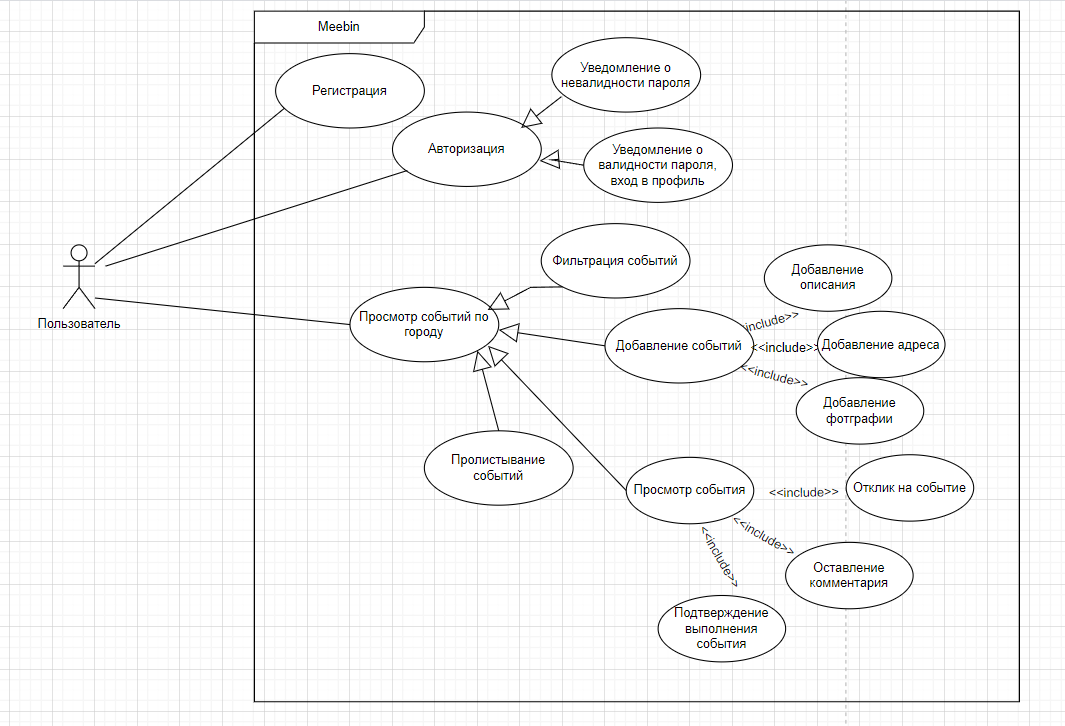
\includegraphics[scale=0.6]{./src/use-case_user.png}}
	\caption{Use-case юзера}
	\label{pic:use-case_user}
\end{figure}

\begin{figure}[H]
	\center{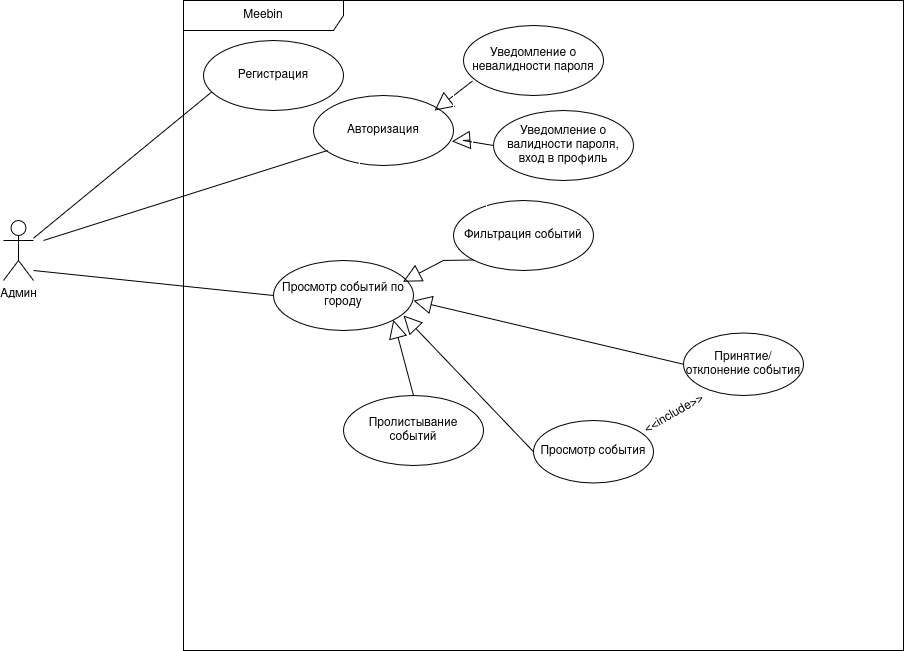
\includegraphics[scale=0.5]{./src/use-case_admin.png}}
	\caption{Use-case админа}
	\label{pic:use-case_admin}
\end{figure}

Как и было сказано выше, основными отличиями в возможностях юзера и админа 
являются их различия в отношении событий: юзер может создавать, но не может 
модерировать, а модератор, в свою очередь, должен лишь отсматривать материал
на предмет правильности.

Рассмотрим детали основных случаев использования приложения.

\subsubsection{Регистрация пользователя}

Прежде чем воспользоваться функционалом приложения, пользователю необходимо 
пройти регистрацию. Этот процесс включает в себя создание аккаунта с указанием 
имени пользователя, электронной почты и пароля. 

Регистрация необходима для того, чтобы обеспечить пользователям возможность 
создания заявок, а также контроля за своими действиями, участия в уборке 
территорий и прочим взаимодействии с другими участниками процесса.

\subsubsection{Создание события}

После регистрации и входа в приложение пользователь может создать событие, 
которое представляет собой заявку на уборку мусора. Пользователь может 
указать все необходимые данные проблемы: описание, точный адрес 
места, а также географические координаты (при помощи GPS или карты). 

После ввода всех данных пользователь отправляет заявку, которая сохраняется 
в базе данных приложения и становится доступной для модерации. Таким образом, 
каждый пользователь может легко и оперативно заявить о мусоре, который 
скопился на улице, и инициировать его уборку. 

\subsubsection{Модерация заявки}

Для обеспечения достоверности информации все созданные пользователями заявки 
проходят этап модерации. Модераторы приложения проверяют, соответствует ли 
указанная информация действительности, и корректно ли описано место 
загрязнения. Это позволяет избежать возможных ошибок или дублирования заявок. 
После проверки заявка либо подтверждается и становится видимой для 
всех пользователей приложения, либо отклоняется, если выявлены несоответствия.

\subsubsection{Просмотр и выбор заявки пользователями}

После подтверждения заявки модератором, она появляется в общем списке активных 
заявок на уборку. Пользователи приложения могут просматривать эти заявки 
как в виде списка, так и на карте, где все места загрязнений будут отмечены 
специальными метками. В этом интерфейсе каждый пользователь может выбрать ту 
заявку, которая ему удобна по расположению или времени проведения уборки. 
После выбора заявки пользователь может принять её для выполнения. Это 
означает, что он берёт на себя ответственность за уборку данного участка, 
и статус заявки меняется на «Принята». Таким образом, другие пользователи 
видят, что заявка уже находится в процессе выполнения, и могут либо 
присоединиться, либо выбрать другую заявку.

\subsubsection{Выполнение уборки и закрытие заявки}

Когда пользователь принимает заявку на выполнение, он отправляется на место 
для проведения уборки. После завершения уборки он загружает в приложение 
фотографии, подтверждающие выполнение работы, и отправляет их на проверку 
модератору. Эти фотографии являются доказательством того, что мусор был 
убран, и заявка может быть закрыта. После загрузки фотографий пользователь 
нажимает кнопку «Заявка выполнена», и статус заявки изменяется на «Завершена».
Модератор проверяет предоставленные материалы, и если всё в порядке, заявка 
окончательно закрывается и исчезает из списка активных задач.

\section{Архитектура приложения}

Архитектура приложения, построенного с использованием Golang, представляет
собой современный и популярный подход к созданию веб-приложений. Это приложение 
может быть ориентировано на создание и управление RESTful API, что делает его 
подходящим для широкого спектра задач, от небольших сервисов до масштабных 
систем.

Хотя в Golang фреймворки не так масштабно влияют на создание приложений, 
Gin-gonic облегчает некоторую реализацию роутинга и работы с построением слоя
контроллера, что в случае использования стандартной библиотеки было бы чуть 
более накладно.

В целом, как и было упомянуто во введении, основной целью является создание 
масштабируемого и архитектурно удобного для поддержки решения. При 
backend-приложения за основу был взят паттерн controller-service-repository,
который применяется для разграничения ответственности и уменьшения сцепленности
между компонентами приложения. Так, при изменении какого-либо участка кода 
(например, при переходе на другую базу данных или изменении бизнес-требований) 
малая сцепленность позволит не переписывать много кода, что уменьшает 
вероятность появления новых ошибок.

Также с целью улучшения дизайна архитектуры на стороне backend-сервиса были 
реализованы следующие концепции:
\begin{enumerate}
    \item Dependency Injection container (DI-container): этот архитектурный 
    паттерн позволяет автоматизировать создание новых сущностей;
    \item паттерн, предложенный компанией <<Авито>> и носящий название 
    Tx-manager, который отвечает за грамотную работу с транзакциями без 
    появления большого количества шаблонного кода \cite{txmanager};
    \item Автоматизация миграций с помощью отдельного контейнера-мигратора.
    При запуске контейнера с backend-сервисами (БД и сервер) также поднимается
    контейнер-мигратор, который автоматически накатывает все имеющиеся локально
    в репозитории миграции. Это как автоматизирует разработку при изменении 
    схемы базы данных, так и помогает при деплое приложения на сторонний сервер.
    \item Для безопасности была использована популярная связка из двух 
    JWT-токенов — access- и refresh-токен.
\end{enumerate}

% \cite{restapi}.

\subsection{Архитектуры базы данных}

\begin{figure}[H]
	\center{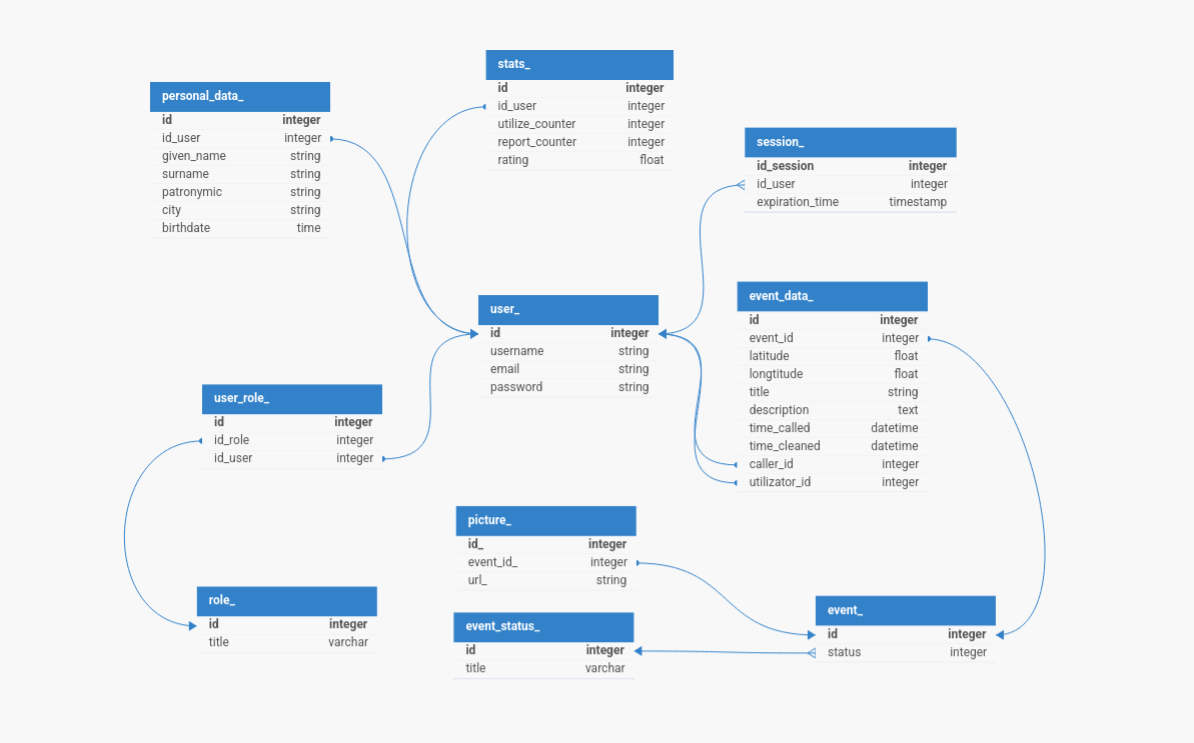
\includegraphics[scale=0.5]{./src/database.png}}
	\caption{Схема базы данных}
	\label{pic:database}
\end{figure}

На данном скриншоте представлена ER-диаграмма создаваемого сервиса. Основные
сущности приложения, как видно, это user\_ (пользователи) и event\_ (события). 
Для большего удобства пользования endpoint-ами API схема была 
нормализована, а также слишком большие таблицы разобраны на несколько других.

Так, данные о пользователе (персональные данные, статистика, информация о 
сессиях) хранятся в разных таблицах. В то же время, если в разбиении 
прямой необходимости нет, то таблица оставляется
большой, поскольку реляционные операции JOIN усложняют построение запроса.

Также с помощью отношения many-to-many была реализована ролевая система, 
которая позволяет администратору модерировать создаваемые пользователями заявки.

В таблице event\_status\_, как и было сказано выше, будет описано 4 стадии события.

\subsection{Архитектура backend-сервиса}

В приложении \ref{appendA} представлена основная 
структура проекта, которая следует одному из наиболее популярных шаблонов, 
подробно описанному в репозитории GitHub под названием \texttt{project-layout} 
\cite{go-project-layout}.

В приложении \ref{appendB} представлен код как backend-, так и 
frontend-приложений. Далее опишем файлы в подробности, останавливаясь на самых 
важных деталях реализации.

\subsubsection{API. Слой контроллера}

Основная задача слоя контроллера, согласно концепции слоистой архитектуры,
обрабатывать запросы от внешних клиентов. Он не должен производить какие-либо 
манипуляции над получаемой сущностью, а также вызывать какие-либо части 
приложения, кроме сервисного (где уже происходит обработка бизнес-логики).

В приложении все контроллеры хранятся в директории \texttt{api}, где 
распределены по трём группам:
\begin{enumerate}
    \item Auth — аутентификация в приложении;
    \item Event — endpoint-ы, связанные с событиями;
    \item User — endpoint-ы, связаннные с пользователями.
\end{enumerate}

Рассмотрим реализацию некоторых концепций.

В файле \texttt{handler.go} представлена функция высшего порядка, принимающая
функцию типа \texttt{func(c *gin.Context) error} и возвращающая функцию типа
\texttt{gin.Handler}. Это делается с целью возможности обработчиком передавать
ошибки в виде возвращаемого значения, которые впоследствии будут использоваться
для сигнализации клиенту API о том, что что-то пошло не так.

Вышеизложенное обусловленно тем, что в Golang ошибка является обычным типом,
который может возвращаться из функции. Это позволяет разработчику возвращать 
более детальную информацию об ошибке при взаимодействии с клиентом.

Рассмотрим также файл \texttt{errors.go}, где создаётся кастомный тип ошибки,
который впоследствии можно передавать в формате JSON:

\begin{minted}[linenos, breaklines=true, style=bw]{Golang}
type Error struct {
    StatusCode int   `json:"-"`
    Message    any   `json:"message"`
    Err        error `json:"-"`
}

func newError(statusCode int, err error, message any) *Error {
    return &Error{
        StatusCode: statusCode,
        Message:    message,
        Err:        err,
    }
}

func NewNotFoundError(err error, message any) *Error {
    return newError(http.StatusNotFound, err, message)
}
\end{minted}

В коде выше на строчке 7 находится функция, создающая объект ошибки, объявленный
в структуре выше. На строчке 15 находится функция, использующая конструктор 
\texttt{func newError} и использующая порождающий паттерн <<фабричный метод>>,
который скрывает создание базового класса ошибки и делегирует это более общим
функциям.

Это позволяет работать с ошибками легко, возвращая нужный код ошибки лишь 
вызовом определённой функции из этого пакета.

Рассмотрим один из хендлеров: остальные устроены по похожей логике с некоторыми
особенностями относительно каждой из CRUD-операций (создание, удаление, 
обновления, получение), а также особенностями авторизации, которые будут 
рассмотрены позднее.

\begin{minted}[linenos, breaklines=true, style=bw]{Golang}
func (h *Handler) Create(c *gin.Context) error {
    ctx := c.Request.Context()
    callerId, ok := c.Get(shared.UserIDJsonName)
    if !ok {
        return api.NewInternalError(nil)
    }
    event := &dto.NewEvent{}
    err := c.ShouldBindJSON(event)
    if err != nil {
        return api.NewBadRequestError(err, api.ParseValidationErrors(err))
    }

    serviceEvent := converter.NewEventServiceToDTO(event)
    eventId, err := h.eventService.Create(ctx, callerId.(uint64), serviceEvent)
    if err != nil {
        switch {
        case errors.Is(err, service.ErrDuplicate):
            return api.NewDuplicateError(err, "Event already exists")
        default:
            return api.NewInternalError(err, "Internal Error")
        }
    }
    c.JSON(http.StatusCreated, dto.IdResponse{Id: eventId})
    return nil
}
\end{minted}

В функции выше на строчке 3-11 происходит валидация данных, определённая в 
функции \texttt{api.ParseValidationErrors}. Затем конвертер (также иногда
называется маппером) переводит сущность DTO (data-transfer object), используемой
в слое API, в сервисную сущность, используемую в слое бизнес-логики или сервиса.

Затем, с уже имеющейся сущностью, тип который подходит для передачи в сервисный
слой, вызывается метод сервисного слоя, который требуется выполнить. В нашем
случае мы хотим создать событие на основе того, что нам было передано в 
теле запроса и что мы уже обработали выше.

Этот паттерн будет и дальше прослеживаться при передаче данных из одного слоя 
в другой.

На строчках 15-22 понятным образом проверяется, вернулось ли какое-либо
значение ошибки из сервисного слоя (если да, то метод не смог завершить свою 
работу успешно и требует обработки исключительной ситуации).

На последних двух строчках с помощью параметра типа \texttt{*gin.Context} 
формируется ответ на запрос клиента в виде JSON-объекта, полями которого 
являются лишь одно значение ID нового объекта события.

\subsubsection{Документация API}

В части документации API располагается автосгенерированная документация с 
помощью утилиты \textit{swag}. Её генерация основывается на комментариях, 
оставленных рядом с методами в программе. Так, комментарии ниже
\begin{minted}[linenos, breaklines=true, style=bw]{go}
// @Tags Auth
// @Summary Login
// @Schemes http
// @Description Creates new pair of refresh-access tokens based on your credentials
// @Accept json
// @Produce json
// @Param LoginCreds body dto.LoginCreds true "Login info"
// @Success 200 {object} dto.ResponseTokens
// @Failure 400 {object} api.Error
// @Failure 401 {object} api.Error
// @Failure 404 {object} api.Error
// @Failure 500 {object} api.Error
// @Router /auth/login [post]
\end{minted}
генерируют следующую документацию
\begin{figure}[H]
	\center{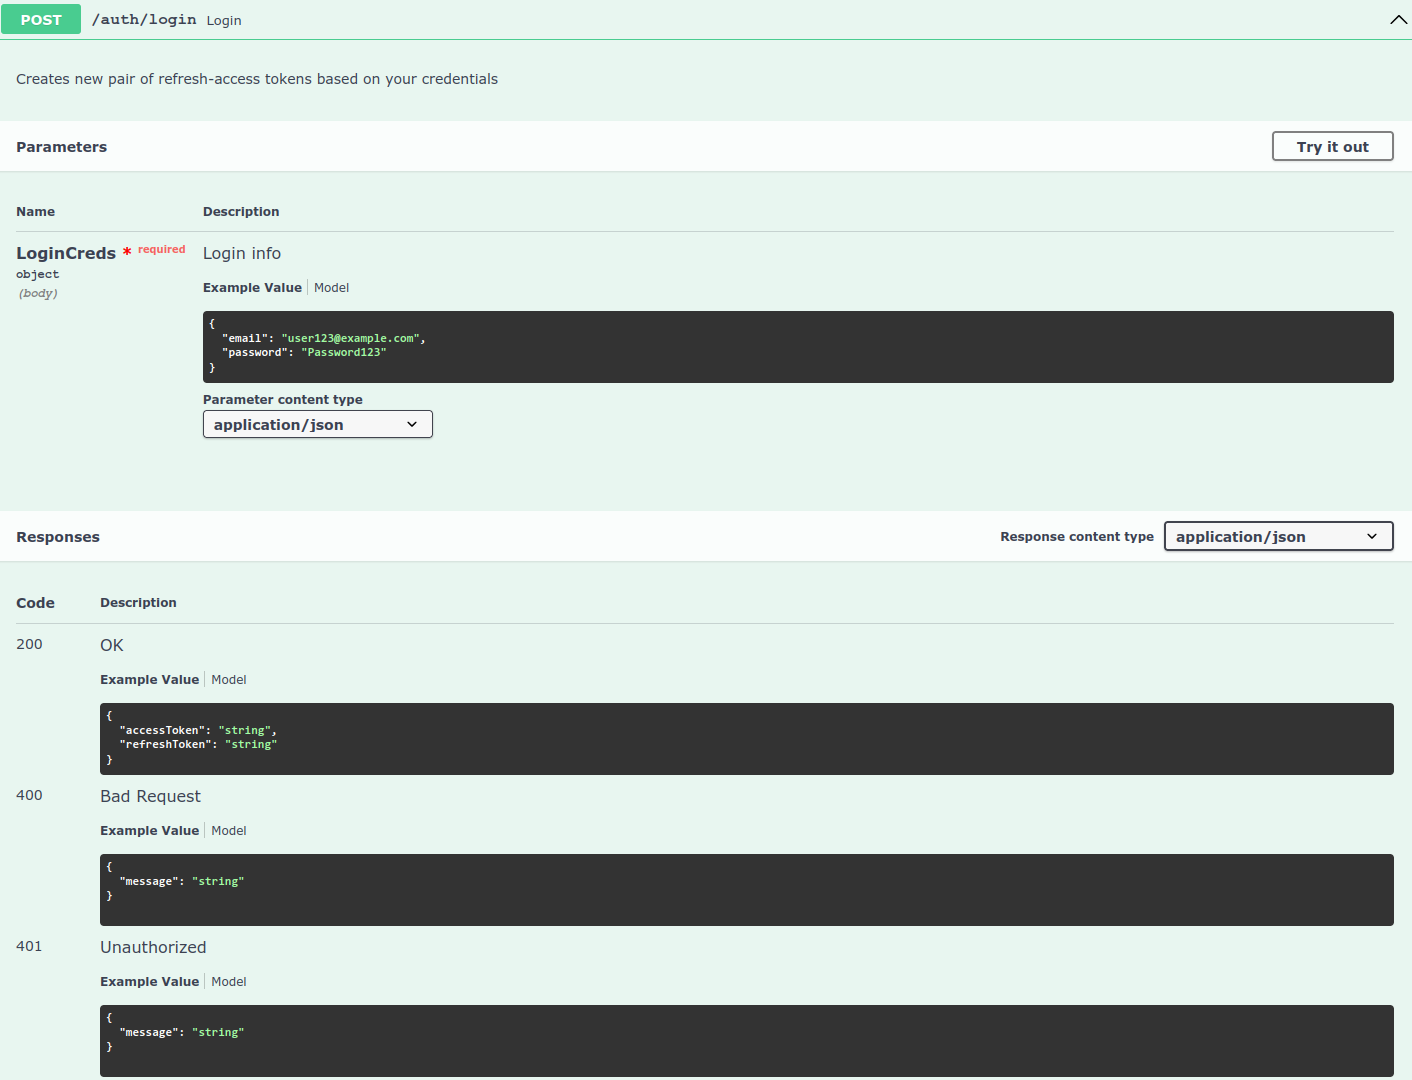
\includegraphics[scale=0.32]{./src/doc_example.png}}
	\caption{Пример документации}
	\label{pic:doc_example}
\end{figure}

Документация генерируется на основе swagger версии 2.0 и содержит следующие 
endpoint:

\begin{figure}[H]
	\center{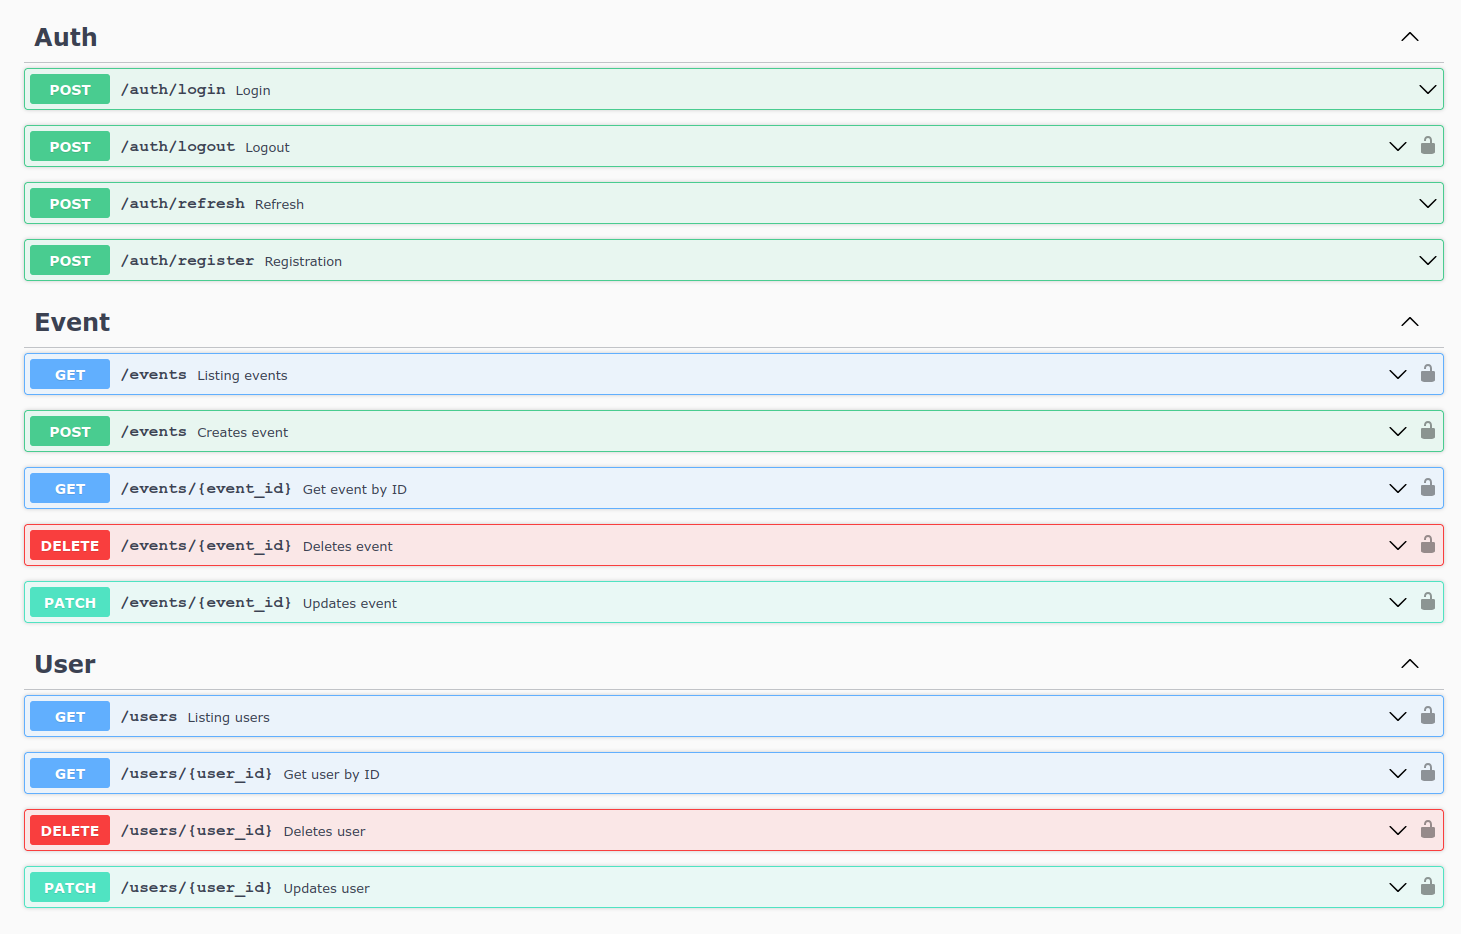
\includegraphics[scale=0.32]{./src/doc_endpoints.png}}
	\caption{Доступные endpoint-ы API}
	\label{pic:doc_endpoints}
\end{figure}

В целом, вся документация API для её последующего предоставления 
Frontend-разработчику генерируется в соответствии с описанием самого пакета
\texttt{Swaggo} в репозитории, указанном в теоретической части.

\subsubsection{Сервис. Слой бизнес-логики}

В слое бизнес-логики обрабатывается приём информации от слоя контроллера и, при
необходимости, происходит взаимодействие с БД посредством слоя репозитория.

Приведём пример логики одной из сервисных функций. Следует отметить, что после 
каждого действия проверяется возвращаемая ошибка (что соответствует 
идиоматичному написанию кода в Golang). В описании алгоритма это опускается. 

В функции \texttt{login} происходят следующие вычисления:
\begin{enumerate}
    \item выполняется поиск в БД по данному email;
    \item если пользователя не существует, то функция вернёт ошибку в контроллер;
    \item выполняется проверка паролей: сверение правильности того, что был 
    отправлен в запросе, и того, который находился в базе данных.
    \item при успешном вводе пароля начинается транзакция в базе данных, в 
    рамках которой:
    \begin{enumerate}
        \item фиксируется время \texttt{refreshExpirationDate}, в которое 
        начата транзакция;
        \item на основе зафиксированного времени вычисляется время окончания 
        refresh-токена;
        \item модель сессии в соответствии со схемой БД \ref{pic:database} 
        передаётся в слой репозитория для сохранения; 
        \item с помощью вынесенной функции создаётся сущность типа JWT 
        refresh-токена для последующей передачи клиенту;
        \item проверяются роли пользователя;
        \item аналогично пункту \textit{г} создаётся access-токен
    \end{enumerate}
    \item в контроллер передаётся пара access- и refresh-токенов.
\end{enumerate}

Таким образом, данная функция реализует алгоритм создания связки двух токенов,
которые впоследствии будут использованы пользователем. Для этого внутри неё
вызываются все вспомогательные функции, которые требуются, а также используются
зависимости. Так, у \texttt{authService} есть зависимости:
\begin{enumerate}
    \item userRepository — репозиторий, отвечающий за таблицу пользователей в БД;
	\item sessionRepository — репозиторий, отвечающий за таблицу сессий в БД;
	\item roleRepository — репозиторий, отвечающий за таблицу ролей в БД;
	\item jwtConfig — позволяет получать данные о текущей конфигурации
    JWT-токенов в приложении;
	\item txManager — позволяет начинать транзакции в БД.
\end{enumerate}

Аналогично этой функции, каждый остальной use-case предполагает наличие 
отдельного метода в сервисном слое. 

\subsubsection{Репозиторий. Слой работы с БД}

В слое репозитория хранится логика взаимодействия приложения с базой данных 
(в нашем случае Postgres). Продолжим рассмотрение примера с функцией логина
и отобразим алгоритм, по которому действует метод репозитория.

В сервисном слое использовались методы поиска пользователей по базе, 
добавления сессии и проверки ролей. Остановимся на рассмотрении последнего:

Сначала сформируем SQL-запрос с помощью библиотеки squirrel:
\begin{minted}[linenos, breaklines=true, style=bw]{go}
query, args, err := sq.Select(
        rep.RoleColumnTitle,
    ).
    PlaceholderFormat(sq.Dollar).
    From(rep.UserRoleTableName).
    LeftJoin(fmt.Sprintf("%s ON %s = %s",
        rep.RoleTableName,
        rep.Col(rep.UserRoleTableName, rep.UserRoleColumnIdRole),
        rep.Col(rep.RoleTableName, rep.RoleColumnId),
        ),
    ).Where(sq.Eq{rep.Col(rep.UserRoleTableName, rep.UserRoleColumnIdUser): userId}).
    ToSql()
\end{minted}

В итоге получаем следующий запрос:
\begin{minted}[linenos, breaklines=true, style=bw]{sql}
    SELECT title 
    FROM user_role_
    LEFT JOIN role_ ON user_role_.id = role_.id
    WHERE user_role_.id = $1
\end{minted}

В запросах SQL, строящихся в backend-приложении и использующих язык SQL, часто
используются плейсхолдеры, которые используют механику параметризованных 
запросов SQL. В нашем случае — это \texttt{\$1}, что означает, 
что аргумент 1, переданные в качестве переменной в метод репозитория. Таким 
образом, вместо плейсхолдера подставится значение того userId (строчка 11 кода 
конструктора запроса), который был передан в метод репозитория.

Таким образом параметризованные запросы и плейсхолдеры, использующиеся здесь,
позволяют избежать потенциальных SQL-инъекций, которые могут повредить 
нашу информационную систему.

Итого, алгоритм работы метода следующий:
\begin{enumerate}
    \item по вышеописанному плану составить запрос;
    \item сделать запрос к базе данных с помощью кастомного клиента к Postgres;
    \item создать массив ролей;
    \item в цикле получать очередной результат (строку) из ответа по запросу в 
    базу данных и добавлять это в массив ролей;
    \item вернуть массив ролей в сервисный слой, который, согласно запросу, 
    описаннному выше, возвращает роли пользователя по данному userId.
\end{enumerate}

Аналогично работают все методы репозитория. При возникновении каких-то 
ошибок нетехнического характера (например, <<такой записи нет>>, или <<запись 
уже существует>>) возвращается кастомная ошибка, которая впоследствии 
обрабатывается в сервисном слое.

\subsubsection{Схемы данных и миграции. Инициализация БД}

Согласно схеме базы данных \ref{pic:database} были составлены миграции, 
которые можно применить к БД и которые изменяют её схему на соответствующую
нашей. Рассмотрим одну из них:

\begin{minted}[linenos, breaklines=true, style=bw]{sql}
-- +goose Up
-- +goose StatementBegin
CREATE TABLE event_data_ (
    id SERIAL PRIMARY KEY,
    event_id INTEGER NOT NULL REFERENCES event_(id) ON DELETE CASCADE,
    latitude FLOAT NOT NULL,
    longtitude FLOAT NOT NULL,
    title VARCHAR(255) NOT NULL,
    description_ TEXT,
    time_called TIMESTAMP,
    time_utilized TIMESTAMP,
    caller_id INTEGER REFERENCES user_(id) ON DELETE NO ACTION,
    utilizator_id INTEGER REFERENCES user_(id) ON DELETE NO ACTION
)
-- +goose StatementEnd

-- +goose Down
-- +goose StatementBegin
DROP TABLE event_data_;
-- +goose StatementEnd
\end{minted}

Это миграция, изначально созданная инструментом Goose и затем описанная 
нами на языке SQL. Также Goose поддерживает описание схемы базы данных на 
языке Golang.

Такие миграции описаны в директории \texttt{backend/migrations} и автоматически
применяются к базе данных при поднятии контейнера мигратора.
Контейнер мигратора выглядит следующим образом:
\begin{minted}[linenos, breaklines=true, style=bw]{Dockerfile}
FROM alpine:latest

RUN apk update && \
    apk upgrade && \
    apk add bash && \
    rm -rf /var/cache/apk/*

ADD https://github.com/pressly/goose/releases/download/v3.24.1/goose_
linux_x86_64 /bin/goose
RUN chmod +x /bin/goose

WORKDIR /root

ADD migrations/*.sql migrations/
ADD migration.sh .
ADD .env .

RUN chmod +x migration.sh

ENTRYPOINT ["bash", "migration.sh"]
\end{minted}

Создаётся минимальный жизнеспособный контейнер, который способен
использовать инструмент \texttt{Goose}. Рассмотрим скрипт, который используется
при запуске контейнера — \texttt{migration.sh}:
\begin{minted}[linenos, breaklines=true, style=bw]{bash}
#!/bin/bash
source .env
export MIGRATION_DSN="host=$DB_HOST port=$PG_PORT dbname=$PG_DB user=$PG_USER password=$PG_PASSWORD"
sleep 2 && goose -dir "${MIGRATION_DIR}" postgres "${MIGRATION_DSN}" up -v
\end{minted}

Этот bash-скрипт позволяет контейнеру применить все данные, 
которые соответствуют нашей базе данных, а также попытаться применить все 
миграции с помощью установленной в контейнер утилиты Goose. Особенность, 
по причине которой мы указываем таймаут запуска скрипта мы рассмотрим в части 
про контейнеризацию.

\subsubsection{Контейнеризация с помощью Docker и Docker compose}

Опишем более детально процесс контейнеризации, который создан для деплоя 
приложения на любом устройстве. Для этих целей, как было сказано в 
теоретической части, используется docker-compose файлы, облегчающие работу с
несколькими контейнерами.

Рассмотрим docker-compose файл, поднимающий backend-сервис, базу данных и 
мигратор:
\begin{minted}[linenos, breaklines=true, style=bw]{yaml}
services:
    db:
      image: postgres:17
      container_name: meebin_db
      restart: unless-stopped
      environment:
        POSTGRES_USER: ${PG_USER}
        POSTGRES_PASSWORD: ${PG_PASSWORD}
        POSTGRES_DB: ${PG_DB}
      ports: 
        - ${PG_PORT}:5432
      volumes:
        - postgres_data:/var/lib/postgresql/data
  
    server:
      container_name: meebin_server_bin
      build:
        context: .
        dockerfile: Dockerfile.bin
      depends_on:
        - db
      ports:
        - ${HTTP_PORT:-8080}:${HTTP_PORT:-8080}
      restart: unless-stopped
  
    migrator:
      container_name: migrator
      build:
        context: .
        dockerfile: Dockerfile.migration
      restart: on-failure
  
  volumes:
    postgres_data:
\end{minted}

В этом файле описано три сервиса, использующие переменные окружения, описанные
в файле .env, а также условия зависимости и перезапуска контейнеров.

Следует обосновать, почему нам не следует указывать условием запуска контейнера
зависимость от контейнера Postgres, как это сделано у backend-сервиса. Так как
запуск контейнера и запуск самой базы данных в контейнере — это не одновременные
и не тождественные понятия, то мы не можем указать просто зависимость от 
контейнера и оставить мигратор без перезапуска. Если мигратор выключится и не 
применит миграции к базе данных, то он не выполнит свою цель. В то же время
backend-сервис может ожидать <<поднятия>> базы данных в своём сервисе, поскольку
это лишь приостановит выполнение запроса на его endpoint-ах в момент обращения
к базе данных.

Решение — это повторяющийся каждый N-период времени скрипт применения миграций.
Как раз это и обеспечивает bash-команда \texttt{sleep 2}.

Таким образом, применение команды \texttt{docker-compose} запустит как 
наши контейнеры с базой данных и backend-сервисом, так и мигратор.

Также для разработки полезен hot-reload server, который бы пересобирал 
приложение при каждом изменении в коде. Это обеспечивает сервер Air, описанный
выше и позволяющий не пересобирать контейнер каждый раз, когда изменяется 
какой-либо элемент кода. Ознакомиться с \texttt{docker-compose.air.yml} файлом 
можно в приложении \ref{appendB}.

\subsection{Архитектура frontend-сервиса}

asd

\subsubsection{Маршрутизация и управление навигацией}

\subsubsection{Обработка авторизации и аутентификации (JWT, OAuth)}

\subsubsection{Интеграция с REST API и обработка запросов}

\section{Использование приложения}

Рассмотрим практическое использование приложение в нескольких сценариях.

\subsection{Регистрация}

\subsection{Логин}

\subsection{Просмотр профиля, редактирование данных}

\subsection{Просмотр событий}

\subsection{Создание событий}

asd

% \begin{figure}[H]
% 	\center{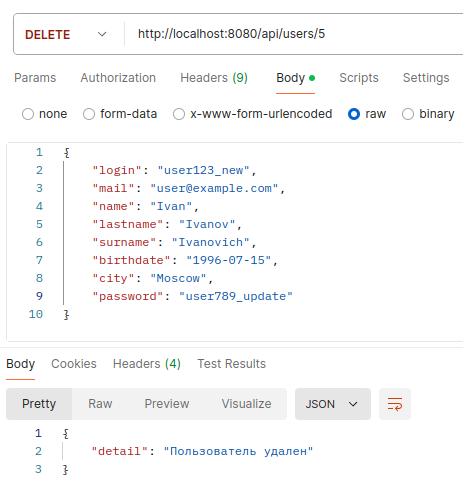
\includegraphics[scale=0.7]{./src/postman_delete_user.png}}
% 	\caption{Запрос на удаление пользователя}
% 	\label{pic8}
% \end{figure}

\conclusion

В ходе выполнения данной дипломной работы были выполнены следующие задачи:
\begin{enumerate}
    \item рассмотреть технологии, описать преимущества выбранного стека;
    \item описать архитектуру и структуру построенной информационной систем;
    \item разработать и продемомстрировать веб-приложение.
\end{enumerate}

Таким образом, все поставленные задачи были выполнены.

Разработанное приложение представляет собой важный шаг в борьбе 
с загрязнением городской среды, объединяя усилия жителей для решения этой 
актуальной проблемы. Тем не менее, будущее данного проекта притом, что 
минимальный жизнеспособный продукт (minimal viable product — MVP), 
выполняющий главный бизнес-процесс, готов, достаточно перспективно и может 
предполагать, например:
\begin{enumerate}
    \item проверка другого жизненного процесса событий с меньшей модерацией;
    \item расширение на другие города с возможностью разделения модерации по 
    городам;
    \item внедрение технологий глубокого обучения для отмены модерации как 
    таковой и её делегирование нейронным сетям;
    \item внедрение систем оповещения либо с помощью нативных оповещений 
    браузера, либо с помощью телеграм-бота.
\end{enumerate}

Таким образом, существуют хорошие перспективы работы над приложением и 
дальше для улучшения возможности решения существующих проблем общества, 
описанных выше. Приложение имеет потенциал для увеличения осведомлённости 
населения о проблемах экологии и вовлечения граждан в активные действия по 
улучшению своей окружающей среды.

\nocite{*}

\inputencoding{cp1251}
\bibliographystyle{gost780uv}
\bibliography{thesis.bib}
\inputencoding{utf8}

\appendix

\section{Структура проекта}
\label{appendA}

% \begin{center}
% \textbf{backend/app/auth.py}
% \end{center}

\begin{minted}[breaklines=true, style=bw]{bash}
.
|— bin
|   |— goose
|   |— minimock
|— cmd
|   |— http_server
|       |— main.go
|— docker-compose.air.yml
|— docker-compose.bin.yml
|— Dockerfile.air
|— Dockerfile.bin
|— Dockerfile.migration
|— docs
|   |— docs.go
|   |— swagger.json
|   |— swagger.yaml
|— go.mod
|— go.sum
|— internal
|   |— api
|   |   |— auth
|   |   |   |— api_auth.go
|   |   |   |— login.go
|   |   |   |— logout.go
|   |   |   |— refresh.go
|   |   |   |— register.go
|   |   |— constants.go
|   |   |— errors.go
|   |   |— event
|   |   |   |— api_event.go
|   |   |   |— create.go
|   |   |   |— delete.go
|   |   |   |— get.go
|   |   |   |— list.go
|   |   |   |— update.go
|   |   |— handler.go
|   |   |— user
|   |   |   |— api_user.go
|   |   |   |— delete.go
|   |   |   |— get.go
|   |   |   |— list.go
|   |   |   |— update.go
|   |   |— validation.go
|   |— app
|   |   |— app.go
|   |   |— closer
|   |   |   |— closer.go
|   |   |— init.go
|   |   |— routes.go
|   |   |— server
|   |   |   |— validator.go
|   |   |— service_provider.go
|   |— client
|   |   |— db
|   |       |— db.go
|   |       |— pg
|   |       |   |— client.go
|   |       |   |— pg.go
|   |       |— transaction
|   |       |   |— transaction.go
|   |       |— transaction.go
|   |— config
|   |   |— config.go
|   |   |— env
|   |   |   |— http.go
|   |   |   |— jwt.go
|   |   |   |— pg.go
|   |   |— env.go
|   |— converter
|   |   |— api
|   |   |   |— event
|   |   |   |   |— base
|   |   |   |   |   |— to_dto.go
|   |   |   |   |   |— to_service.go
|   |   |   |   |— create
|   |   |   |   |   |— to_service.go
|   |   |   |   |— update
|   |   |   |       |— to_service.go
|   |   |   |— token
|   |   |   |   |— to_dto.go
|   |   |   |— user
|   |   |       |— base
|   |   |       |   |— to_dto.go
|   |   |       |   |— to_service.go
|   |   |       |— login
|   |   |       |   |— to_service.go
|   |   |       |— register
|   |   |       |   |— to_service.go
|   |   |       |— update
|   |   |           |— to_dto.go
|   |   |           |— to_service.go
|   |   |— role.go
|   |   |— service
|   |       |— event
|   |       |   |— to_repo.go
|   |       |   |— to_service.go
|   |       |— user
|   |           |— to_repo.go
|   |           |— to_service.go
|   |— middleware
|   |   |— auth.go
|   |— model
|   |   |— event
|   |   |   |— dto
|   |   |   |   |— base.go
|   |   |   |   |— create.go
|   |   |   |   |— id.go
|   |   |   |   |— update.go
|   |   |   |— r_model
|   |   |   |   |— event.go
|   |   |   |— s_model
|   |   |       |— event.go
|   |   |— role.go
|   |   |— status.go
|   |   |— token
|   |   |   |— dto
|   |   |       |— tokens.go
|   |   |— user
|   |       |— dto
|   |       |   |— base.go
|   |       |   |— login.go
|   |       |   |— register.go
|   |       |   |— update.go
|   |       |— r_model
|   |       |   |— user.go
|   |       |— s_model
|   |           |— user.go
|   |— repository
|   |   |— errors.go
|   |   |— event
|   |   |   |— add.go
|   |   |   |— delete.go
|   |   |   |— get.go
|   |   |   |— list.go
|   |   |   |— repository.go
|   |   |   |— update.go
|   |   |— repository.go
|   |   |— role
|   |   |   |— find.go
|   |   |   |— repository.go
|   |   |— session
|   |   |   |— add.go
|   |   |   |— find.go
|   |   |   |— remove.go
|   |   |   |— repository.go
|   |   |— sql_names.go
|   |   |— user
|   |       |— add.go
|   |       |— delete.go
|   |       |— get_creds.go
|   |       |— get_user.go
|   |       |— list.go
|   |       |— repository.go
|   |       |— update.go
|   |— service
|   |   |— auth
|   |   |   |— helper
|   |   |   |   |— helper.go
|   |   |   |— login.go
|   |   |   |— logout.go
|   |   |   |— refresh.go
|   |   |   |— register.go
|   |   |   |— service.go
|   |   |— constants.go
|   |   |— errors.go
|   |   |— event
|   |   |   |— add.go
|   |   |   |— delete.go
|   |   |   |— get.go
|   |   |   |— list.go
|   |   |   |— service.go
|   |   |   |— update.go
|   |   |— service.go
|   |   |— user
|   |       |— delete.go
|   |       |— get.go
|   |       |— list.go
|   |       |— service.go
|   |       |— update.go
|   |— shared
|       |— jwt.go
|— Makefile
|— migrations
|   |— 20250224182407_create_user_table.sql
|   |— 20250224183811_create_personaldata_table.sql
|   |— 20250224184716_create_userstats_table.sql
|   |— 20250224185347_create_session_table.sql
|   |— 20250224185654_create_roles_table.sql
|   |— 20250224185804_create_userrole_table.sql
|   |— 20250307190708_create_basic_roles.sql
|   |— 20250325071118_create_event_status_table.sql
|   |— 20250325071213_create_event_table.sql
|   |— 20250325071433_create_event_data_table.sql
|— migration.sh
|— README.md
\end{minted}

\section{USB-носитель с кодом написанного приложения}
\label{appendB}
На приложенном USB-носителе можно ознакомиться со следующими файлами:
\begin{description}
\item[Директория \texttt{backend}] — backend-приложение;
\begin{description}
    \item[Файл \texttt{cmd/http\_server/main.go}] — стартовая точка 
    backend-приложения;
    \item[Директория \texttt{docs}] — содержит файлы о документации API 
    приложения;
    \item[Директория \texttt{internal}] — содержит код, описывающий логику 
    работы сервера;
    \begin{description}
        \item[Директория \texttt{api}] — директория, связанная с обслуживанием 
        клиент-серверного взаимодействия;
        \item[Директория \texttt{app}] — директория, связанная с дизайном 
        архитектуры, абстракциями и запуском основной сущности приложения;
        \item[Директория \texttt{client}] — директория, связанная с кастомным 
        клиентом к базе данных;
        \item[Директория \texttt{config}] — директория, связанная с 
        исходной конфигурацией и настройкой параметров приложения;
        \item[Директория \texttt{converter}] — директория, связанная с 
        конвертированием моделей с одного слоя в другой;
        \item[Директория \texttt{middleware}] — директория, связанная с 
        middleware, используемыми в API;
        \item[Директория \texttt{model}] — директория сущностей бизнес-логики;
        \item[Директория \texttt{repository}] — директория, связанная с 
        обслуживанием получения данных из хранящего слоя (БД);
        \item[Директория \texttt{service}] — директория, реализующая 
        бизнес-логику;
        \item[Директория \texttt{shared}] — директория, содержащая 
        переиспользуемые в более чем одном пакете структуры и константы;
    \end{description}
    \item[Директория \texttt{migrations}] — содержит SQL-миграции базы данных
    \item[Файл \texttt{.env}] — содержит параметры конфигурации, подгружаемые 
    при запуске приложения;
    \item[Файлы с префиксом \texttt{docker-compose}] — содержат YAML-
    конфигурацию автоматического запуска контейнеров в stack'е;
    \item[Файлы с префиксом \texttt{Dockerfile}] — содержат информацию о 
    кастомных образах, на основе которых создаются контейнеры;
    \item[Файл \texttt{migration.sh}] — описывает используемый в контейнере 
    мигратора скрипт для автоматической накатки миграций;
    \item[Файлы с префиксом \texttt{go}] — используются компилятором Go для 
    обслуживания зависимостей проекта;
    \item[Файл \texttt{Makefile}] — используется для автоматизации работы с 
    консольными командами, используемыми в проекте;
\end{description}

\item[Директория \texttt{frontend}] — frontend-приложение;
\begin{description}
    \item[Директория \texttt{app}] — содержит основные компоненты приложения,
    а также файлы конфигурации frontend-приложения;
    \begin{description}
        \item[Директория \texttt{components}]
        \item[Директория \texttt{hooks}]
        \item[Директория \texttt{routes}]
    \end{description} 
\end{description}
\end{description}

\end{document}
